\documentclass[12pt]{article}

\usepackage[margin=1.0in]{geometry}
\usepackage{tikz}
\usepackage{tabto}
\usetikzlibrary{automata,positioning}
\usepackage{enumitem}
\usepackage{amsmath}
\usepackage{amssymb}
\usetikzlibrary{automata,positioning}

\begin{document}

\title{CS4384 : Automata Theory\\Homework Assignment 4}
\author{Matthew McMillian\\mgm160130@utdallas.edu}
\maketitle

\begin{enumerate}
	\item For each of the following languages, say whether it is context-free. If so, write a CFG or draw a PDA (non-mathematically) that generates the language. If not, prove it using the pumping lemma and/or closure properties for CFLs. \\
	\begin{itemize}
		\item[a.)] L = $\{a^{n^2}$ $|$ $n \geq 0 \}$ \\ \\
		Assume L is a context free language and let p be its pumping length. Let S be a partitioning of a string in the language L such that S = $a^{p^2}$, and let S be defined in a way that satisfies the pumping lemma conditions $|$vxy$|$ $\leq$ p and $|$vy$|$ $>$ 0.  Choose i = 0, such that S$^{'}$ = uv$^i$xy$^i$z $\rightarrow$ uxz. Since $|$vy$|$ $>$ 0, we know that either v or y contains an a $\in$ L's alphabet., thus S$^{'}$ = $a^{p^2 - 1}$, which is not necessarily in the language. Since we have pumped a string in the language and found that S$^{'}$ $\not \in$ L, this contradicts the pumping lemma, and we conclude that L is not context free. \\
		
		\item[b.)] L = $\{a^m b^n c^{(m-n)}$ $|$ $m \geq n \}$ \\ \\
		We can define a PDA (seen below) that accepts the language L, this L is context free. \\ \\
		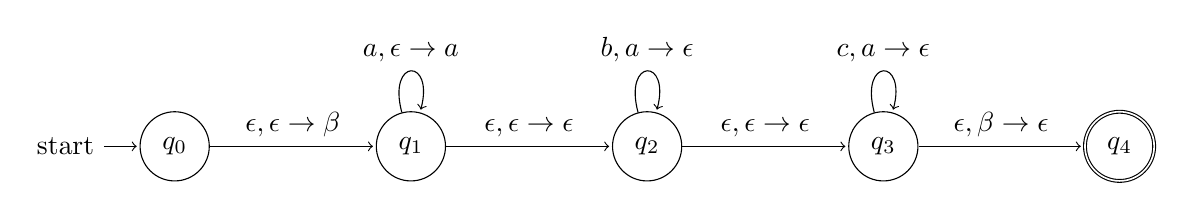
\begin{tikzpicture}[shorten >=1pt,node distance=3cm,on grid,auto] 
   \node[state,initial] (q_0)   {$q_0$}; 
   \node[state] (q_1) [right=of q_0] {$q_1$}; 
   \node[state] (q_2) [right=of q_1] {$q_2$}; 
   \node[state](q_3) [right=of q_2] {$q_3$};
   \node[state, accepting](q_4) [right=of q_3] {$q_4$};
    \path[->] 
    (q_0) edge node {$\epsilon, \epsilon \rightarrow \beta$} (q_1)
    (q_1) edge node {$\epsilon, \epsilon \rightarrow \epsilon$} (q_2)
    	  edge [loop above] node {$a, \epsilon \rightarrow a$} (q_1)
    (q_2) edge node {$\epsilon, \epsilon \rightarrow \epsilon$} (q_3)
    	  edge [loop above] node {$b, a \rightarrow \epsilon$} (q_2)
    (q_3) edge node {$\epsilon, \beta \rightarrow \epsilon$} (q_4)
    	  edge [loop above] node {$c, a \rightarrow \epsilon$} (q_3);
\end{tikzpicture} \\

	\item[c.)] L = $\{a^m b^n c^{mn}$ $|$ $m, n \geq 0 \}$ \\ \\
	Assume L is a context free language and let p be its pumping length. Let S be a partitioning of a string in the language L such that S = $a^pb^pc^{p^2}$, and let S be defined in a way that satisfies the pumping lemma conditions $|$vxy$|$ $\leq$ p and $|$vy$|$ $>$ 0.  Choose i = 0, such that S$^{'}$ = uv$^i$xy$^i$z $\rightarrow$ uxz. We consider 2 cases in order to analyze the string S$^{'}$. Since $|$vy$|$ $>$ 0, we know that v and/or y must contain a character, and since $|$vxy$|$ $\leq$ p we know that v,y can only be an a or b. Notice that if v,y contain any character character $\in$ $\Sigma$. If v,y are the any character, then we obtain strings like S$^{'}$ = a$^{p - v_l}$b$^{p - y_l}$c$^{p^2}$, where $v_l$, $y_l$ are the length of subsections v and y respectively. Notice since $|$vy$|$ $>$ 0, $v_l$, $y_l$ must be at least one (for one of the subsections). Thus, $p - v_l$ * $p - y_l$ $\not =$ $p^2$, therefore the string is not in the language. Since we have pumped a string in the language and found that S$^{'}$ $\not \in$ L, this contradicts the pumping lemma, and we conclude that L is not context free. \\
	
	\item[d.)] L = $\{a^n b^n c^m$ $|$ $m > n \}$ \\ \\
	Assume L is a context free language and let p be its pumping length. Let S be a partitioning of a string in the language L such that S = $a^pb^pc^{p+1}$, and let S be defined in a way that satisfies the pumping lemma conditions $|$vxy$|$ $\leq$ p and $|$vy$|$ $>$ 0. Choose i = 2, such that S$^{'}$ = uv$^i$xy$^i$z $\rightarrow$ uv$^2$xy$^2$z. Since $|$vy$|$ $>$ 0 we know that v or y must contain an element, and since $|$vxy$|$ $\leq$ p we know that v,y can only be an a or b based on our partitioning. Consider the three cases below:
	\begin{itemize}
		\item [Case 1:] v,y contain the same element(s). If v,y contain the same element(s), then trivially we can see a$^{p + v_l + y_l}$b$^{p}$ or a$^{p}$b$^{p + v_l + y_l}$ is not strictly less than $p+1$, where $v_l$, $y_l$ are the length of subsections v and y respectively. Thus, this fails the pumping lemma.
		\item [Case 2:] v,y contain different element(s). Trivially we can see that v,y contain different elements of different lengths then the partitioning and subsequently the pumping lemma fails. If they are the same length, we can see that a$^{p+v_l}$b$^{p+y_l}$ is not strictly less than $p+1$, thus this case fails the pumping lemma.
	\end{itemize}
	 Since we have pumped a string in the language and found that S$^{'}$ $\not \in$ L based on multiple cases, this contradicts the pumping lemma, and we conclude that L is not context free. \\	
	\end{itemize}
	
	\item Define R(L) = $\{s^r$ $|$ $s \in L\}$ That is, R(L) is the language of all strings that are reverses of strings in L. Prove that R is the closure property of CFLs. \textit{(Hint: Assume there exists a CFG in CNF that generates L, and use it to mathematically define a new CFG that generates R(L)).} \\ \\
	Consider a CFG in CNF defined by G = (V,$\Sigma$,R,S). Since we know G is in CNF, we know that G does not contain a mix of terminals and non-terminals. Consider G$^{'}$ = (V,$\Sigma$,R$_{reversed}$,S) such that R$_{reversed}$ is equal to the set of rules consisting of $<$left$>$ $\rightarrow$ $<$right$>$, but reversed to $<$left$>$ $\rightarrow$ $<$right$_{reversed}>$. Since G is in CNF, we know that no non-terminals and terminals are mixed, thus if we reverse the right side, we will get anything G can create but reversed. \\
	
	\item Define C(L1, L2) = $\{s1s2$ $|$ $s1 \in L1, s2 \in L2, |s1| = |s2| \}$ That is, C(L1, L2) is a special kind of language concatenation in which only the equal-length strings in L1 and L2 are paired together. Prove that if L1 and L2 are both regular languages, then C(L1, L2) is a CFL. (\textit{Hint: Assume there exist DFAs A1 and A2 accepting L1 and L2, respectively, and use them to mathematically define a PDA that accepts C(L1, L2)).} \\ \\
	We can define a new PDA below that accepts C(L1, L2). \\
	Q : The set of states = $\{q_0, q_1\}$ \\
	$\Sigma^*$: The alphabet defined by $\Sigma_{L1}$ $\bigcup$ $\Sigma_{L2}$ \\
	$\Gamma$: The alphabet of the stack = $\Sigma^*$ \\
	$\delta$: The set of transitions given by $\{((q, q+1), \Sigma_{L1})$ $|$ $q \in Q_{L1}, q+1 \in Q_{L2}\}$ $\bigcup$ \tabto{6.15cm} $\{((q, q+1), \Sigma_{L2})$ $|$ $q \in Q_{L2}, q+1 \in Q_{L1}\}$ \\
	q$_0$ $\in$ Q: The starting state \\
	F $\subset$ Q: The accepting states s.t. the state number mod 2 = 0. \\
	Thus, we have proven that C(L1, L2) is a CFL. \\
	
	\item PDAs with two stacks are strictly more powerful than PDAs with one stack. Prove
that 2-stack PDAs are not a valid model for CFLs by giving an example of a language that
is not context free and yet accepted by a 2-stack PDA. Describe (no math necessary) how a
2-stack PDA would accept that language. \\ \\
	Consider the language L = $\{a^nb^nc^n$ $|$ $n \geq 0\}$, which we know to be non-context-free since we proved it in class. Now consider this 2-stack PDA given below. \\ \\
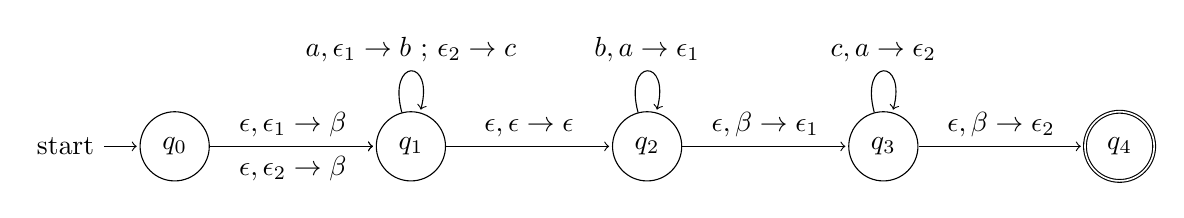
\begin{tikzpicture}[shorten >=1pt,node distance=3cm,on grid,auto] 
   \node[state,initial] (q_0)   {$q_0$}; 
   \node[state] (q_1) [right=of q_0] {$q_1$}; 
   \node[state] (q_2) [right=of q_1] {$q_2$}; 
   \node[state](q_3) [right=of q_2] {$q_3$};
   \node[state, accepting](q_4) [right=of q_3] {$q_4$};
    \path[->] 
    (q_0) edge [above] node {$\epsilon, \epsilon_1 \rightarrow \beta$} (q_1)
    	  edge [below] node {$\epsilon, \epsilon_2 \rightarrow \beta$} (q_1)
    (q_1) edge node {$\epsilon, \epsilon \rightarrow \epsilon$} (q_2)
    	  edge [loop above] node {$a, \epsilon_1 \rightarrow b$ ; $\epsilon_2 \rightarrow c$} (q_1)
    (q_2) edge node {$\epsilon, \beta \rightarrow \epsilon_1$} (q_3)
    	  edge [loop above] node {$b, a \rightarrow \epsilon_1$} (q_2)
    (q_3) edge node {$\epsilon, \beta \rightarrow \epsilon_2$} (q_4)
    	  edge [loop above] node {$c, a \rightarrow \epsilon_2$} (q_3);
\end{tikzpicture} \\ \\
Here we have defined a 2-stack PDA that accepts our non-context free language. On each operation, the stack may either push or pop 2 elements from either stack. In this case, we show how this wouldn't work by pushing two elements onto two stacks at the same time, which allows us to pop twice separately from each stack until we reach our accepting state. 	This is problematic since our PDA acceptes a language that is not context free.
		
\end{enumerate}


\end{document}